\documentclass{article}

\usepackage{graphicx}
\usepackage{amsmath}
\usepackage{amssymb}
\usepackage{caption}

\renewcommand{\figurename}{Figura}

\begin{document}

\begin{flushleft}
    \LARGE Banjercito \\[6pt]
    \Large Diplomado en Ciencia de Datos
\end{flushleft}

\vfill

\begin{flushleft}
    \LARGE \textbf{Tarea 502} \\[12pt]
    \LARGE Módulo V | Semana 1 \\[24pt]
\end{flushleft}

\vfil

\begin{flushleft}
    Alan Badillo Salas \\[12pt]
    Noviembre 2024 \\[24pt]
\end{flushleft}

\vfill

\section*{Introducción}
El Diplomado en Ciencia de Datos ha llegado a su quinto módulo titulado "\textit{Deep Learning}". En este módulo revisaremos a profundidad las redes neuronales generales, recurrentes y convolutivas para resolver problemas generales y particulares de forma automática, mejorando así la predicción y pronóstico en los análisis y casos de estudio relacionados.
\\[12pt]
En la semana 1 hemos hecho un repaso sobre los temas más importantes de los módulos anteriores, partiendo del uso de Python, Numpy y Pandas, así como la probabilidad y estadística bayesiana y de los modelos de Regresión y Clasificación de Machine Learning. También se introdujo el concepto de \textit{Perceptrón} y su aplicación para predecir un objetivo a través de sus características.
\\[12pt]
En esta tarea se reforzarán las habilidades para hacer un análisis probabilístico y estadístico con Excel y Python.

\clearpage

\section*{Tarea 502 | Probabilidad y Estadística de Deuda}

Una financiera posee una lista de 30 créditos no completados que fueron otorgados a clientes de diferente edad, escolaridad, años de servicio y si eran casados. La financiera requiere entender algunas probabilidades y estadísticos descriptivos de los datos.
\\[12pt]
Genera una hoja de Excel que contenga los siguientes datos sobre los 30 créditos otorgados y la deuda total de cada cliente:

\begin{table}[h!]
    \centering
    \begin{tabular}{|c|r|r|c|c|c|c|}
        \hline
        Cliente & Crédito & Deuda & Edad & Escolaridad & Años & Casado \\
        \hline
        1  & \$5,000.00  & \$800.00  & 25 & Preparatoria & 1  & 0 \\
        2  & \$6,000.00  & \$200.00  & 25 & Licenciatura & 2  & 0 \\
        3  & \$8,000.00  & \$3,500.00 & 27 & Preparatoria & 1  & 0 \\
        4  & \$9,000.00  & \$3,000.00 & 28 & Licenciatura & 3  & 1 \\
        5  & \$10,000.00 & \$2,500.00 & 29 & Preparatoria & 2  & 0 \\
        6  & \$12,000.00 & \$6,000.00 & 26 & Preparatoria & 1  & 1 \\
        7  & \$12,000.00 & \$3,000.00 & 24 & Preparatoria & 3  & 0 \\
        8  & \$13,000.00 & \$2,500.00 & 26 & Licenciatura & 2  & 0 \\
        9  & \$15,000.00 & \$4,000.00 & 31 & Preparatoria & 1  & 0 \\
        10 & \$15,000.00 & \$500.00  & 33 & Licenciatura & 2  & 1 \\
        11 & \$16,000.00 & \$3,000.00 & 34 & Licenciatura & 2  & 0 \\
        12 & \$17,000.00 & \$1,500.00 & 40 & Licenciatura & 5  & 0 \\
        13 & \$19,000.00 & \$800.00  & 36 & Licenciatura & 5  & 1 \\
        14 & \$19,000.00 & \$1,200.00 & 34 & Maestría    & 3  & 0 \\
        15 & \$20,000.00 & \$900.00  & 42 & Licenciatura & 7  & 1 \\
        16 & \$23,000.00 & \$6,000.00 & 48 & Maestría    & 5  & 0 \\
        17 & \$23,000.00 & \$13,000.00 & 52 & Licenciatura & 12 & 0 \\
        18 & \$23,000.00 & \$4,000.00 & 54 & Licenciatura & 5  & 1 \\
        19 & \$25,000.00 & \$5,000.00 & 36 & Maestría    & 8  & 0 \\
        20 & \$25,000.00 & \$9,000.00 & 39 & Licenciatura & 5  & 0 \\
        21 & \$26,000.00 & \$8,000.00 & 41 & Licenciatura & 2  & 1 \\
        22 & \$27,000.00 & \$14,000.00 & 56 & Licenciatura & 24 & 0 \\
        23 & \$28,000.00 & \$6,000.00 & 54 & Maestría    & 5  & 1 \\
        24 & \$28,000.00 & \$8,000.00 & 28 & Licenciatura & 3  & 1 \\
        25 & \$30,000.00 & \$6,000.00 & 31 & Licenciatura & 6  & 1 \\
        26 & \$34,000.00 & \$7,000.00 & 58 & Licenciatura & 12 & 0 \\
        27 & \$34,000.00 & \$8,000.00 & 64 & Preparatoria & 24 & 1 \\
        28 & \$35,000.00 & \$8,000.00 & 66 & Maestría    & 40 & 0 \\
        29 & \$35,000.00 & \$6,000.00 & 56 & Preparatoria & 36 & 1 \\
        30 & \$35,000.00 & \$12,000.00 & 58 & Licenciatura & 28 & 1 \\
        \hline
    \end{tabular}
    \caption{Datos de clientes}
    \label{tab:datos_clientes}
\end{table}

\clearpage

\hfil\\
Calcula los conteos siguientes:
\begin{itemize}
    \item Número total de clientes que están casados
    \item Número de clientes menores o iguales a 30 años
    \item Número de clientes entre 31 y 39 años
    \item Número de clientes entre 40 y 55 años
    \item Número de clientes mayores o iguales a 56 años
    \item Número de clientes con Preparatoria
    \item Número de clientes con Licenciatura
    \item Número de clientes con Maestría
    \item Número de clientes con 1 o 2 años de servicio
    \item Número de clientes con 3 a 5 años de servicio
    \item Número de clientes con 6 o más años de servicio
\end{itemize}
Calcula las siguientes probabilidades (porcentaje de que ocurra):
\begin{itemize}
    \item Probabilidad que un cliente esté casado
    \item Probabilidad que un cliente tenga hasta 30 años
    \item Probabilidad que un cliente tenga entre 31 y 39 años
    \item Probabilidad que un cliente tenga entre 40 y 55 años
    \item Probabilidad que un cliente tenga al menos 56 años
    \item Probabilidad que un cliente tenga Preparatoria
    \item Probabilidad que un cliente tenga Licenciatura
    \item Probabilidad que un cliente tenga Maestría
    \item Probabilidad que un cliente tenga 1 o 2 años de servicio
    \item Probabilidad que un cliente tenga de 3 a 5 años de servicio
    \item Probabilidad que un cliente tenga 6 o más años de servicio
\end{itemize}
Calcula los siguientes estadísticos:
\begin{itemize}
    \item Suma de la deuda en crétidos entre \$5,000 y \$10,000
    \item Suma de la deuda en crétidos entre \$11,000 y \$15,000
    \item Suma de la deuda en crétidos entre \$16,000 y \$20,000
    \item Suma de la deuda en crétidos entre \$21,000 y \$25,000
    \item Suma de la deuda en crétidos entre \$26,000 y \$30,000
    \item Suma de la deuda en crétidos entre \$31,000 y \$35,000
    \item La deuda menor en crétidos entre \$5,000 y \$10,000
    \item La deuda menor en crétidos entre \$11,000 y \$15,000
    \item La deuda menor en crétidos entre \$16,000 y \$20,000
    \item La deuda menor en crétidos entre \$21,000 y \$25,000
    \item La deuda menor en crétidos entre \$26,000 y \$30,000
    \item La deuda menor en crétidos entre \$31,000 y \$35,000
    \item La deuda mayor en crétidos entre \$5,000 y \$10,000
    \item La deuda mayor en crétidos entre \$11,000 y \$15,000
    \item La deuda mayor en crétidos entre \$16,000 y \$20,000
    \item La deuda mayor en crétidos entre \$21,000 y \$25,000
    \item La deuda mayor en crétidos entre \$26,000 y \$30,000
    \item La deuda mayor en crétidos entre \$31,000 y \$35,000
    \item Promedio de la deuda en crétidos entre \$5,000 y \$10,000
    \item Promedio de la deuda en crétidos entre \$11,000 y \$15,000
    \item Promedio de la deuda en crétidos entre \$16,000 y \$20,000
    \item Promedio de la deuda en crétidos entre \$21,000 y \$25,000
    \item Promedio de la deuda en crétidos entre \$26,000 y \$30,000
    \item Promedio de la deuda en crétidos entre \$31,000 y \$35,000
    \item Desviación estándar de la deuda en crétidos entre \$5,000 y \$10,000
    \item Desviación estándar de la deuda en crétidos entre \$11,000 y \$15,000
    \item Desviación estándar de la deuda en crétidos entre \$16,000 y \$20,000
    \item Desviación estándar de la deuda en crétidos entre \$21,000 y \$25,000
    \item Desviación estándar de la deuda en crétidos entre \$26,000 y \$30,000
    \item Desviación estándar de la deuda en crétidos entre \$31,000 y \$35,000
\end{itemize}
Calcula las siguientes probabilidades conjuntas:
\begin{itemize}
    \item Probabilidad que un cliente tenga hasta 30 años y esté casado
    \item Probabilidad que un cliente tenga hasta 30 años y tenga Preparatoria
    \item Probabilidad que un cliente tenga hasta 30 años y tenga Licenciatura
    \item Probabilidad que un cliente tenga hasta 30 años y tenga Maestría
    \item Probabilidad que un cliente tenga entre 31 y 39 años y esté casado
    \item Probabilidad que un cliente tenga entre 31 y 39 años y tenga Preparatoria
    \item Probabilidad que un cliente tenga entre 31 y 39 años y tenga Licenciatura
    \item Probabilidad que un cliente tenga entre 31 y 39 años y tenga Maestría
    \item Probabilidad que un cliente tenga entre 40 y 55 años y esté casado
    \item Probabilidad que un cliente tenga entre 40 y 55 años y tenga Preparatoria
    \item Probabilidad que un cliente tenga entre 40 y 55 años y tenga Licenciatura
    \item Probabilidad que un cliente tenga entre 40 y 55 años y tenga Maestría
    \item Probabilidad que un cliente tenga al menos 56 años y esté casado
    \item Probabilidad que un cliente tenga al menos 56 años y tenga Preparatoria
    \item Probabilidad que un cliente tenga al menos 56 años y tenga Licenciatura
    \item Probabilidad que un cliente tenga al menos 56 años y tenga Maestría
\end{itemize}
Calcula las siguientes probabilidades condicionales:
\begin{itemize}
    \item Probabilidad que un cliente casado tenga hasta 30 años
    \item Probabilidad que un cliente casado tenga entre 31 y 39 años
    \item Probabilidad que un cliente casado tenga entre 40 y 55 años
    \item Probabilidad que un cliente casado tenga al menos 56 años
    \item Probabilidad que un cliente casado tenga Preparatoria
    \item Probabilidad que un cliente casado tenga Licenciatura
    \item Probabilidad que un cliente casado tenga Maestría
    \item Probabilidad que un cliente con Preparatoria esté casado
    \item Probabilidad que un cliente con Licenciatura esté casado
    \item Probabilidad que un cliente con Maestría esté casado
\end{itemize}
Calcula las siguientes probabilidades condicionales sobre la deuda relativa, es decir, la deuda entre el crédito, por ejemplo, para una deuda de \$800, y un crédito de \$5,000 la deuda relativa es $800/5000 = 0.16 = 16\%$:
\begin{itemize}
    \item Cliente casado que tenga una deuda relativa de hasta 20\%
    \item Cliente casado que tenga una deuda relativa de entre 20\% y 40\%
    \item Cliente casado que tenga una deuda relativa de entre 40\% y 60\%
    \item Cliente casado que tenga una deuda relativa de entre 60\% y 80\%
    \item Cliente casado que tenga una deuda relativa mayor a 80\%
    \item Cliente con Preparatoria que tenga una deuda relativa de hasta 20\%
    \item Cliente con Preparatoria que tenga una deuda relativa de entre 20\% y 40\%
    \item Cliente con Preparatoria que tenga una deuda relativa de entre 40\% y 60\%
    \item Cliente con Preparatoria que tenga una deuda relativa de entre 60\% y 80\%
    \item Cliente con Preparatoria que tenga una deuda relativa mayor a 80\%
    \item Cliente con Licenciatura que tenga una deuda relativa de hasta 20\%
    \item Cliente con Licenciatura que tenga una deuda relativa de entre 20\% y 40\%
    \item Cliente con Licenciatura que tenga una deuda relativa de entre 40\% y 60\%
    \item Cliente con Licenciatura que tenga una deuda relativa de entre 60\% y 80\%
    \item Cliente con Licenciatura que tenga una deuda relativa mayor a 80\%
    \item Cliente con Maestría que tenga una deuda relativa de hasta 20\%
    \item Cliente con Maestría que tenga una deuda relativa de entre 20\% y 40\%
    \item Cliente con Maestría que tenga una deuda relativa de entre 40\% y 60\%
    \item Cliente con Maestría que tenga una deuda relativa de entre 60\% y 80\%
    \item Cliente con Maestría que tenga una deuda relativa mayor a 80\%
\end{itemize}

\clearpage

\hfill\\
Sigue los pasos del \textit{script} para generar distintos reportes sobre las probabilidades conjuntas de estar casado por escolaridad y el porcentaje de deuda relativa por escolaridad.
\\[12pt]
Carga los datos de los créditos con Pandas:
\begin{verbatim}
import pandas
creditos = pandas.read_excel("/content/p502.xlsx")
creditos
\end{verbatim}
\textbf{Pregunta}: ¿Cuál es la deuda máxima de los clientes con Preparatoria?
\\[12pt]
Calula la columna de deuda relativa (deuda entre crédito):
\begin{verbatim}
creditos["Deuda Rel"] = 100 * \
    creditos["Deuda"] / creditos["Crédito"]
creditos
\end{verbatim}
\textbf{Pregunta}: ¿Cuáles son las dos deudas relativas más grandes, qué escolaridad tienen y en qué rango de edad están?
\\[12pt]
Crea un DataFrame para reportar las probabilidades condicionales de que dado que el cliente tiene cierta escolaridad y esté o no casado:
\begin{verbatim}
import numpy
reporteCasadoEscolaridad = pandas.DataFrame(
    numpy.zeros((3, 2)), 
    index=["Preparatoria", "Licenciatura", "Maestria"], 
    columns=["Casado", "No casado"])
reporteCasadoEscolaridad
\end{verbatim}
\textbf{Pregunta}: ¿Por qué se usa $numpy.zeros((3, 2))$?
\\[12pt]
Llena el DataFrame con los conteos usando dos filtros, el primero indicará cual es la escolaridad y el segundo si está casado, se usará la probabilidad condicional $P(B | A) = P(B, A) / P(A)$:
\begin{verbatim}
for escolaridad in ["Preparatoria", "Licenciatura", "Maestria"]:
  for casado, columna in [(1, "Casado"), (0, "No casado")]:
    filtro1 = creditos["Escolaridad"] == escolaridad
    filtro2 = creditos["Casado"] == casado
    proba = len(creditos[filtro1 & filtro2]) / \
        len(creditos[filtro1])
    reporteCasadoEscolaridad.loc[escolaridad, columna] = \
        proba * 100
\end{verbatim}
\textbf{Pregunta}: ¿Cuál es la probabilidad de que un cliente que tiene maestría, no esté casado?
\\[12pt]
Grafica en un pastel para cada escolaridad la probabilidad de estar o no casado:
\begin{verbatim}
import matplotlib.pyplot as pyplot

for escolaridad in ["Preparatoria", "Licenciatura", "Maestria"]:
  filtro1 = creditos["Escolaridad"] == escolaridad
  filtro2A = creditos["Casado"] == 1
  filtro2B = creditos["Casado"] == 0
  A = len(creditos[filtro1 & filtro2A])
  B = len(creditos[filtro1 & filtro2B])
  pyplot.pie([A, B], 
             labels=[f"Casado ({A})", f"No casado ({B})"],
             autopct="%.1f%%")
  pyplot.title(f"Cliente con {escolaridad}")
  pyplot.savefig(f"r1-{escolaridad}-casado.png")
  pyplot.show()
\end{verbatim}
En la Figura \ref{fig:escolaridad_casado} observamos las gráficas de pastel que comparar la probabilidad de estar casado por escolaridad.
\begin{figure}[h]
    \centering
    \begin{minipage}{0.3\textwidth}
        \centering
        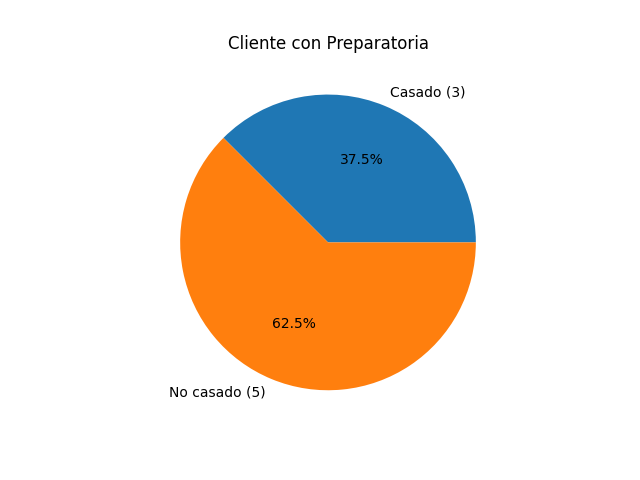
\includegraphics[width=\textwidth]{figures/r1-Preparatoria-casado.png}
    \end{minipage}
    \hfill
    \begin{minipage}{0.3\textwidth}
        \centering
        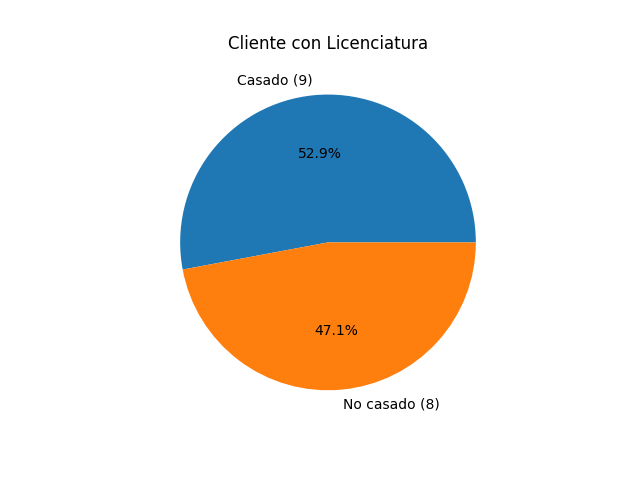
\includegraphics[width=\textwidth]{figures/r1-Licenciatura-casado.png}
    \end{minipage}
    \hfill
    \begin{minipage}{0.3\textwidth}
        \centering
        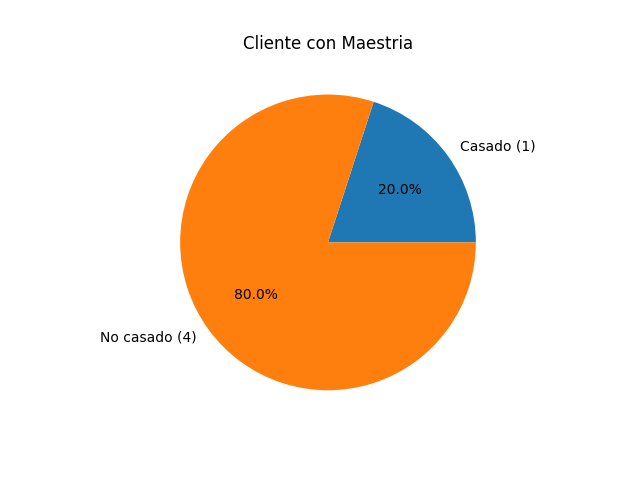
\includegraphics[width=\textwidth]{figures/r1-Maestria-casado.png}
    \end{minipage}
    \captionsetup{width=0.9\textwidth}
    \caption{Probabilidad de estar casado en clientes por escolaridad}
    \label{fig:escolaridad_casado}
\end{figure}
\\[12pt]
\textbf{Pregunta}: ¿Qué escolaridad tienen mayor probabilidad de que un cliente no esté casado y cuál de que si lo esté?
\\[12pt]
Haz un análisis similar para la probabilidad condicional por escolaridad pero ahora para el porcentaje de deuda relativa:
\begin{verbatim}
import numpy

reporteDeudaEscolaridad = pandas.DataFrame(numpy.zeros((3, 6)), 
    index=["Preparatoria", "Licenciatura", "Maestria"], 
    columns=["10%", "20%", "30%", "40%", "50%", "60%"])

for escolaridad in ["Preparatoria", "Licenciatura", "Maestria"]:
    for lim_inf, lim_sup, columna in [(-1, 10, "10%"), 
        (10, 20, "20%"), (20, 30, "30%"), 
        (30, 40, "40%"), (40, 50, "50%"), (50, 100, "60%")]:
      filtro1 = creditos["Escolaridad"] == escolaridad
      filtro2 = creditos["Deuda Rel"] > lim_inf
      filtro3 = creditos["Deuda Rel"] <= lim_sup
      proba = len(creditos[filtro1 & filtro2 & filtro3]) / \
        len(creditos[filtro1])
      reporteDeudaEscolaridad.loc[escolaridad, columna] = \
        proba * 100

reporteDeudaEscolaridad
\end{verbatim}
\textbf{Pregunta}: ¿Cuál es la probabilidad de tener una deuda entre 20\% y 30\% dado que el cliente tiene Maestría y cuál dado que el cliente tiene Preparatoria?
\\[12pt]
Genera una gráfica de mapa de calor sobre los datos del reporte (escolaridad y porcentaje de deuda relativa):
\begin{verbatim}
import seaborn
seaborn.heatmap(reporteDeudaEscolaridad)
pyplot.savefig("escolaridad_deuda_heatmap.png")
\end{verbatim}
En la Figura \ref{fig:escolaridad_deuda_heatmap} se muestra el mapa de calor de la probabilidad de tener cierto porcentaje de deuda relativa por escolaridad:
\begin{figure}[h]
    \centering
    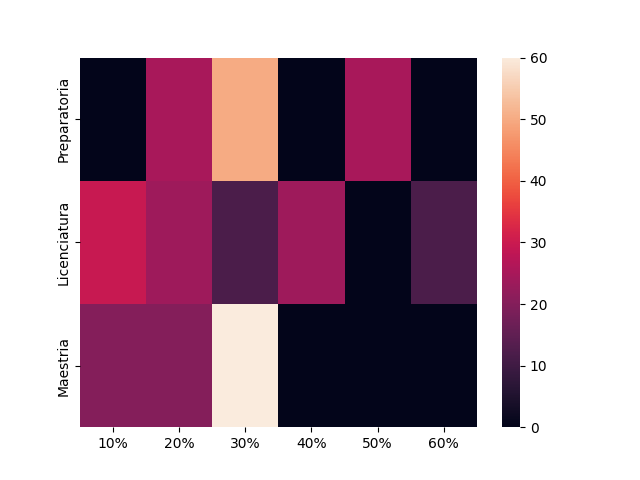
\includegraphics[width=0.8\textwidth]{figures/escolaridad_deuda_heatmap.png}
    \captionsetup{width=\textwidth}
    \caption{Mapa de calor con la escolaridad contra el porcentaje de deuda}
    \label{fig:escolaridad_deuda_heatmap}
\end{figure}
\\[12pt]
\textbf{Pregunta}: ¿Cómo se interpreta esta gráfica, dónde concentra el mayor porcentaje de deduda relativa cada escolaridad?

\clearpage

\hfill\\
Finalmente, crea una representación en gráfica de barras de los mismos datos:
\begin{verbatim}
import matplotlib.pyplot as pyplot

pyplot.bar(
    numpy.arange(len(reporteDeudaEscolaridad.columns)) + 0, 
    reporteDeudaEscolaridad.loc["Preparatoria"],
    label="Preparatoria",
    width=0.2)
pyplot.bar(
    numpy.arange(len(reporteDeudaEscolaridad.columns)) + 0.2, 
    reporteDeudaEscolaridad.loc["Licenciatura"],
    label="Licenciatura",
    width=0.2)
pyplot.bar(
    numpy.arange(len(reporteDeudaEscolaridad.columns)) + 0.4, 
    reporteDeudaEscolaridad.loc["Maestria"],
    label="Maestria",
    width=0.2)

pyplot.xticks(
    numpy.arange(len(reporteDeudaEscolaridad.columns)) + 0.2, 
    reporteDeudaEscolaridad.columns) 

pyplot.title("Deuda Relativa por Escolaridad")
pyplot.xlabel("Deuda Relativa")
pyplot.ylabel("% Créditos")
pyplot.legend()

pyplot.savefig("escolaridad_deuda_bar.png")

pyplot.show()
\end{verbatim}

\clearpage

\hfill\\
En la Figura \ref{fig:escolaridad_deuda_bar} se muestra las barras agrupadas de la probabilidad de tener cierto porcentaje de deuda relativa por escolaridad:
\begin{figure}[h]
    \centering
    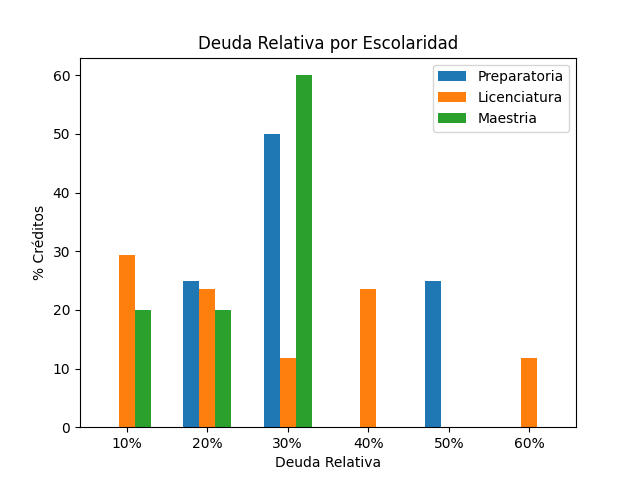
\includegraphics[width=0.8\textwidth]{figures/escolaridad_deuda_bar.png}
    \captionsetup{width=\textwidth}
    \caption{Barras agrupadas con la escolaridad contra el porcentaje de deuda}
    \label{fig:escolaridad_deuda_bar}
\end{figure}
\\[12pt]
\textbf{Pregunta}: ¿Cómo se interpreta esta gráfica, dónde concentra el mayor porcentaje de deduda relativa cada escolaridad?
\\[12pt]
Escribe tus conclusiones y piensa en cómo se haría un análisis por edad en lugar de escolaridad.

\end{document}